\section{\huge{Bonus exercises}}

\subsection{The cozy exercise}

Connect the dots.

\begin{center}
\includegraphics[width=.99\textwidth]{forbind-prikkerne.pdf}
\end{center}


\newpage
\subsection{The ``rus'' exercise}
As this year's ``rus'' did not get to start from Scratch. Cut, write, and
arrange the puzzle such that the cat turns 360°.
\hspace*{-0.15\textwidth}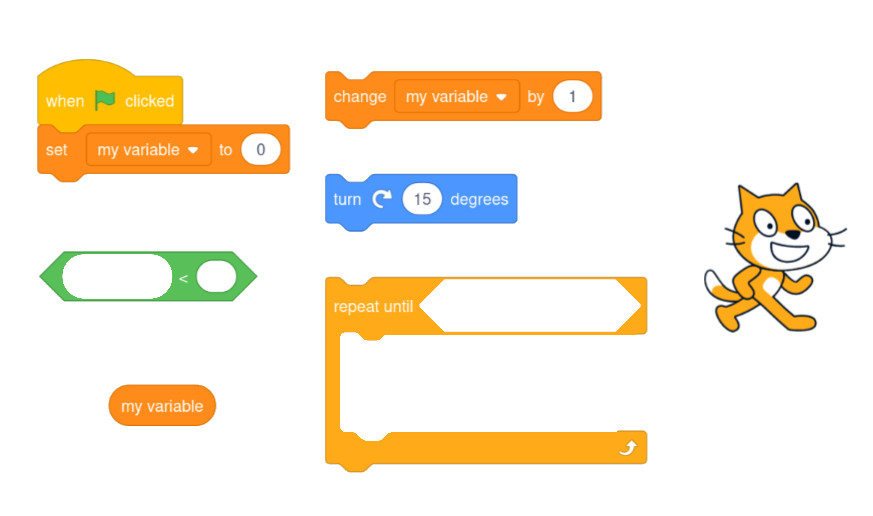
\includegraphics[width=1.3\textwidth]{figures/scratch.jpg}
\vspace{-.9cm}
\subsection{2. year ``rus'' exercise}
\vspace*{-.4cm}
Implement an \verb|AND| circut using \verb|NAND| and \verb|INV|
\vspace*{-.7cm}\\
\begin{center}
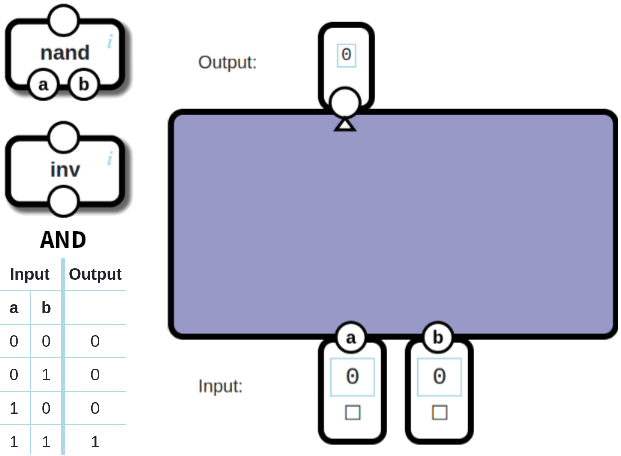
\includegraphics[width=1\textwidth]{figures/compsys.png}
\end{center}

\subsection{3. year exercise}
Assume you chose LICS, but left your book at home. You've drunk the \verb|n|th
bottle of schnaps and you're trying to explain to your friend that god exists
or doesn't. After scrambling for arguments you write the following down:
\begin{align*}
    \frac{P}{P\vee Q}\vee i
    \quad\quad\frac{P\rightarrow \bot}{\neg P}\neg i
    \quad\quad\frac{P,\neg P}{\bot}\neg e
    \quad\quad\frac{\neg\neg\neg P}{\neg P}\neg\neg e
\end{align*}
Now prove that:
\begin{align*}
   \frac{}{P \vee \neg P}
\end{align*}

\subsection{The small exercises}
\vspace{-0.1cm}

\subsubsection{Sub exercise 0}
\vspace{-0.2cm}

Donald likes primes, but only knows the primes up to and including 2. Help him
write a F\# (or SML) function, which will find all primes below 100.

\subsubsection{Sub exercise  1}

Donal loves all IEEE standards equally and has recently found IEE 754 for
representing numbers. Help him rewrite the number $173.8$ to it's 32-bit IEEE
754 representation. Did you loose precision?

\subsubsection{Sub exercise 2}
\vspace{-0.2cm}

Implement a x64 simulator in C.

Indent with spaces and wrap at 79 charaters.

\subsubsection{Sub exercise 3}
\vspace{-0.2cm}

Dry run the following Whitespace-program and report its output:
\begin{verbatim}


\end{verbatim}

\newpage
\subsection{C exercise}
Rewrite the following x86-64 assembly code to C without using \verb|goto|
statements.
\lstdefinelanguage
   [x64]{Assembler}     % add a "x64" dialect of Assembler
   [x86masm]{Assembler} % based on the "x86masm" dialect
   % with these extra keywords:
   {morekeywords={CDQE,CQO,CMPSQ,CMPXCHG16B,JRCXZ,LODSQ,MOVSXD, %
                  POPFQ,PUSHFQ,SCASQ,STOSQ,IRETQ,RDTSCP,SWAPGS, %
                  rax,rdx,rcx,rbx,rsi,rdi,rsp,rbp, %
                  r8,r8d,r8w,r8b,r9,r9d,r9w,r9b, %
                  r10,r10d,r10w,r10b,r11,r11d,r11w,r11b, %
                  r12,r12d,r12w,r12b,r13,r13d,r13w,r13b, %
                  r14,r14d,r14w,r14b,r15,r15d,r15w,r15b}} % etc.
% Skud ud til https://tex.stackexchange.com/questions/51645/x86-64-assembler-language-dialect-for-the-listings-package
\begin{lstlisting}[language={[x64]Assembler}]
program:
    movq (%rdi), %rax
    testq %rax, %rax
    je L1
    addq $8, %rdi
    movq %rax, %rdx
L3:
    cmpq %rdx, %rax
    cmovl %rdx, %rax
    addq $8, %rdi
    movq -8(%rdi), %rdx
    testq %rdx, %rdx
    jne L3
L1:
    ret
\end{lstlisting}
[Compsys exam, 2017]

\textbf{Discuss} Do you feel you better prepared to solve the exercise after
passing ACS?

\subsection{Sudoku}
\begin{center}
    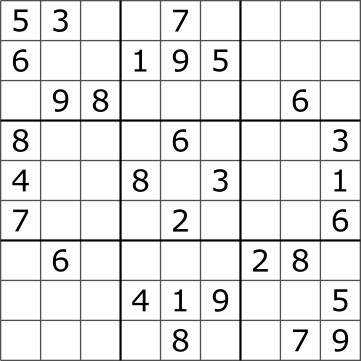
\includegraphics[width=0.65\textwidth]{figures/sudoku.jpg}
\end{center}

\newpage

\subsection{The bearded exercise}

Santa's Quantum-Blockchain-AI-printer has broken down after he got his new
quantum bits from the Physicist. Therefore he can't use it to print the name
tags for all the presents.

Luckily an elf just found his old printer in the garage,
there's just one problem. While it can print a name tag for each child, it has
a bug that means it will print the same name for each present. He decides that
the only fair solution is to pick the name to be the one that is closest to
every child in the worlds name and use that name, then surely no one can
complain. By close he means the number of letters he needs to replace to change
one name into another. So the name Mathias and Matthew would be a distance of 4
from each other, and one name closest to both could be Mathiew, as this is only
2 replacements from each.

\begin{center}
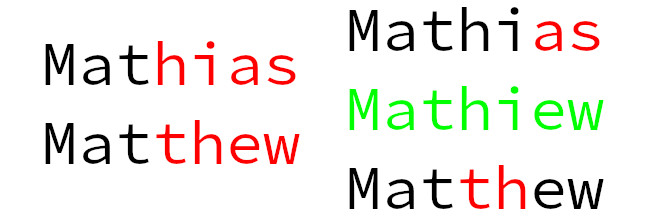
\includegraphics[width=.9\textwidth]{figures/mathias.jpg}
\end{center}

Now he just needs to figure out some way of finding
the name that's closest to the name of every child in the world before the end
of the night so he can get the printer started, and just maybe Christmas can be
saved (read: at most polynomial time).

Feel free to ask the toastmaster for the list of names, but of course they are encrypted so as to apply with GDPR

\vspace{0.5em}\textbf{\emph{NB:\@ The first to solve this exercise and turn in
a correct solution in the bar will win a bottle of homemade schnapps!}}
